\documentclass[a4paper,12pt]{article}
\usepackage{amsmath,amssymb,amsfonts,amsthm}
\usepackage{tikz}
\usepackage [utf8x] {inputenc}
\usepackage [T2A] {fontenc} 
\usepackage[russian]{babel}
\usepackage{cmap} 
\usepackage{gensymb}

% Так ссылки в PDF будут активны
\usepackage[unicode]{hyperref}

% вы сможете вставлять картинки командой \includegraphics[width=0.7\textwidth]{ИМЯ ФАЙЛА}
% получается подключать, как минимум, файлы .pdf, .jpg, .png.
\usepackage{graphicx}
% Если вы хотите явно указать поля:
\usepackage[margin=1in]{geometry}
% Или если вы хотите задать поля менее явно (чем больше DIV, тем больше места под текст):
% \usepackage[DIV=10]{typearea}

\usepackage{fancyhdr}

\newcommand{\bbR}{\mathbb R}%теперь вместо длинной команды \mathbb R (множество вещественных чисел) можно писать короткую запись \bbR. Вместо \bbR вы можете вписать любую строчку букв, которая начинается с '\'.
\newcommand{\eps}{\varepsilon}
\newcommand{\bbN}{\mathbb N}
\newcommand{\dif}{\mathrm{d}}

\newtheorem{Def}{Определение}


\pagestyle{fancy}
\makeatletter % сделать "@" "буквой", а не "спецсимволом" - можно использовать "служебные" команды, содержащие @ в названии
\fancyhead[L]{\footnotesize Термодинамика и молекулярная физика}%Это будет написано вверху страницы слева
\fancyhead[R]{\footnotesize ФМХФ МФТИ}
\fancyfoot[L]{\footnotesize \@author}%имя автора будет написано внизу страницы слева
\fancyfoot[R]{\thepage}%номер страницы —- внизу справа
\fancyfoot[C]{}%по центру внизу страницы пусто

\renewcommand{\maketitle}{%
	\noindent{\bfseries\scshape\large\@title\ \mdseries\upshape}\par
	\noindent {\large\itshape\@author}
	\vskip 2ex}
\makeatother
\def\dd#1#2{\frac{\partial#1}{\partial#2}}


\title{2.5.1 \\ Измерение коэффициента поверхностного натяжения} 
\author{Егор Берсенев} 
\date{2 мая 2016 г.}

\begin{document}
	\maketitle
	\section{Цель:}
	\begin{enumerate}
		\item Измерение коэффициента поверхностного натяжения исследуемой жидкости при разной температуре с использованием известного коэффициента поверхностного натяжения другой жидкости.
		\item Определение полной поверхностной энергии и теплоты, необходимой для изотермического образования единицы поверхности жидкости.
	\end{enumerate}
	\section{Оборудование:}
		Прибор Ребиндера с термостатом, спирт, вода, стаканы.
	\section{Теоретическая часть}
	Наличие поверхностного слоя приводит к различию давлений по разные стороны от искривленной поверхности раздела двух сред. Для сферического пузырька внутри жидкости избыточное давление определяется формулой Лапласа.
	\begin{equation}
		\Delta P = P_1 - P_2 = \frac{2\sigma}{r}
	\end{equation}
	\section{Экспериментальная установка}
	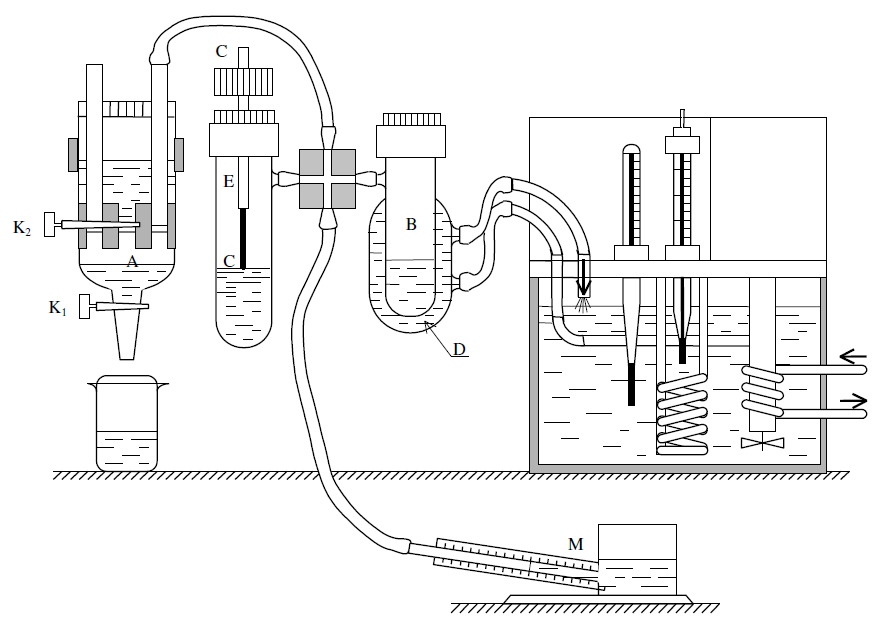
\includegraphics[width = 0.7\linewidth]{instrument}
	\begin{enumerate}
		\item A --- аспиратор, из которого по каплям вытекает вода, создавая разрежение.
		\item В --- сосуд с исследуемой жидкостью.
		\item С --- металлическая игла.
		\item D --- рубашка, поддерживающая температуру термостата в сосуде В.
		\item E --- сосуд с дистиллированной водой.
		\item M --- наклонный манометр.
	\end{enumerate}
	\section{Ход работы}
		Измерим максимальное давление при пробулькивании пузырька в спирте.
	\begin{center}
		\begin{table}[h]
			\begin{tabular}{|l|l|l|l|l|l|l|l|l|l|}
				$P_1$, см  & 44.5 & 45 & 44.5 & 45 & 45 & 45 & 45 & 45 & 45 \\
			\end{tabular}
		\end{table}
	\end{center}
	Оценим диаметр иглы по формуле $(1)$. 
	\[
	d = \frac{4\sigma}{\Delta P} = \frac{4\cdot0.0223}{45\cdot0.2\cdot 9.8}= 1.01\cdot 10^{-3}\,\text{м} = 1.01\,\text{мм}
	\]
	Диаметр иглы полученный прямым измерением равен $d = 1.05 \,\text{мм}$
	Измерим давление на высоте $h_1 = 1.85 \,\text{см}$ при температуре $T = 25 \celsius$
	\begin{center}
		\begin{table}[h]
			\begin{tabular}{|l|l|l|l|l|l|}
				$\Delta P$, дел & 118 & 118 & 118 & 118 & 118 \\
			\end{tabular}
		\end{table}
	\end{center}
	Измерим давление на высоте $h_2 = 0.65 \,\text{см}$ при температуре $T = 25 \celsius$
	\begin{center}
		\begin{table}[h]
			\begin{tabular}{|l|l|l|l|l|l|}
				$\Delta P$, дел & 178 & 178 & 178 & 178 & 178 \\
			\end{tabular}
		\end{table}
	\end{center}
	Оценим глубину погружения по разности давлений:$\Delta(\Delta P) = (178-118)\cdot0.2\cdot9.8 = 117.6 \,\text{Па}$. Теперь оценим давление столба жидкости по прямому измерению высоты: $\Delta h = 1.2\,\text{см} \implies \Delta(\Delta P) = \rho gh = 117.6 \,\text{Па}$. Разности давлений совпали, значит можно проводить измерения.
	
	Теперь проведем измерения $\sigma(T)$.
	\begin{center}
		\begin{table}[h!]
			\begin{tabular}{l|l|l|l|l|l|l|l}
				T, K & 301.1 & 305.1 & 309.1 & 313.2 & 317.2 & 321.2 & 325.2 \\ \hline
	 $\Delta P$, дел & 215 & 214 & 213 & 212 & 210 & 209 & 208 \\
					 & 216 & 214 & 213 & 212 & 211 & 210 & 208 \\
					 & 216 & 214 & 213 & 212 & 210 & 209 & 208 \\
					 & 216 & 214 & 213 & 212 & 210 & 209 & 208 \\
					 & 216 & 214 & 213 & 212 & 211 & 209 & 208 \\ \hline
			$\sigma\cdot 10^{-3}$ Н \ м & 80.3 & 79.3 & 78.8 & 78.3 & 77.5 & 76.7 & 76.2 \\ \hline
			\end{tabular}
		\end{table}
	\end{center}
	
	\begin{center}
		\begin{table}[h!]
			\begin{tabular}{l|l|l}
				T, K & $Q\cdot 10^{-3}$ Дж & $U_\text{п}∕\text{П}\cdot 10^{-3}$ Дж \\ \hline
				301.1 & 50.27 & 130.6 \\
				305.1 & 50.93 & 130.2 \\
				309.1 & 51.60 & 130.4 \\
				313.2 & 52.29 & 130.6 \\
				317.2 & 52.95 & 130.5 \\
				321.2 & 53.62 & 130.3 \\
				325.2 & 54.29 & 130.5 \\ \hline

			\end{tabular}
		\end{table}
	\end{center}
	
	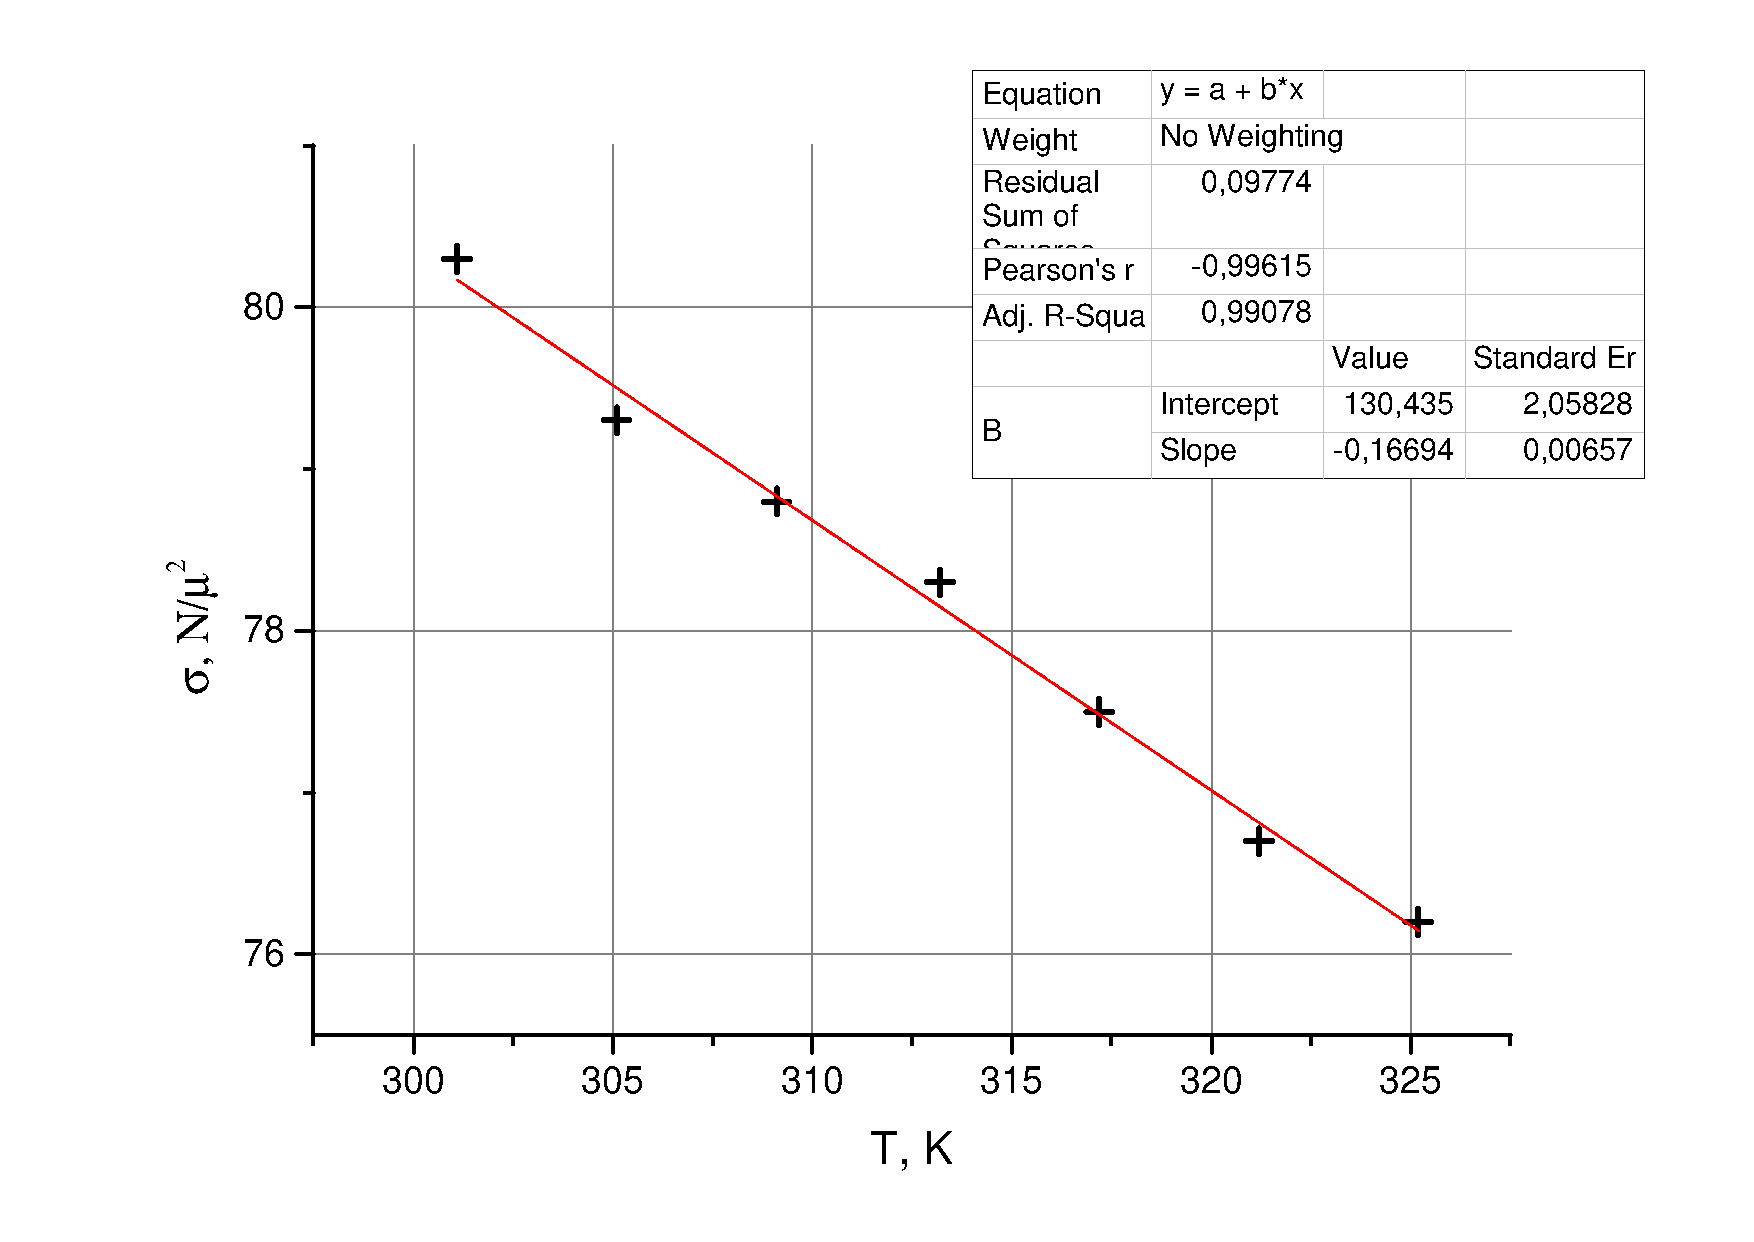
\includegraphics[width = 0.7\linewidth]{sigmaT}
	
	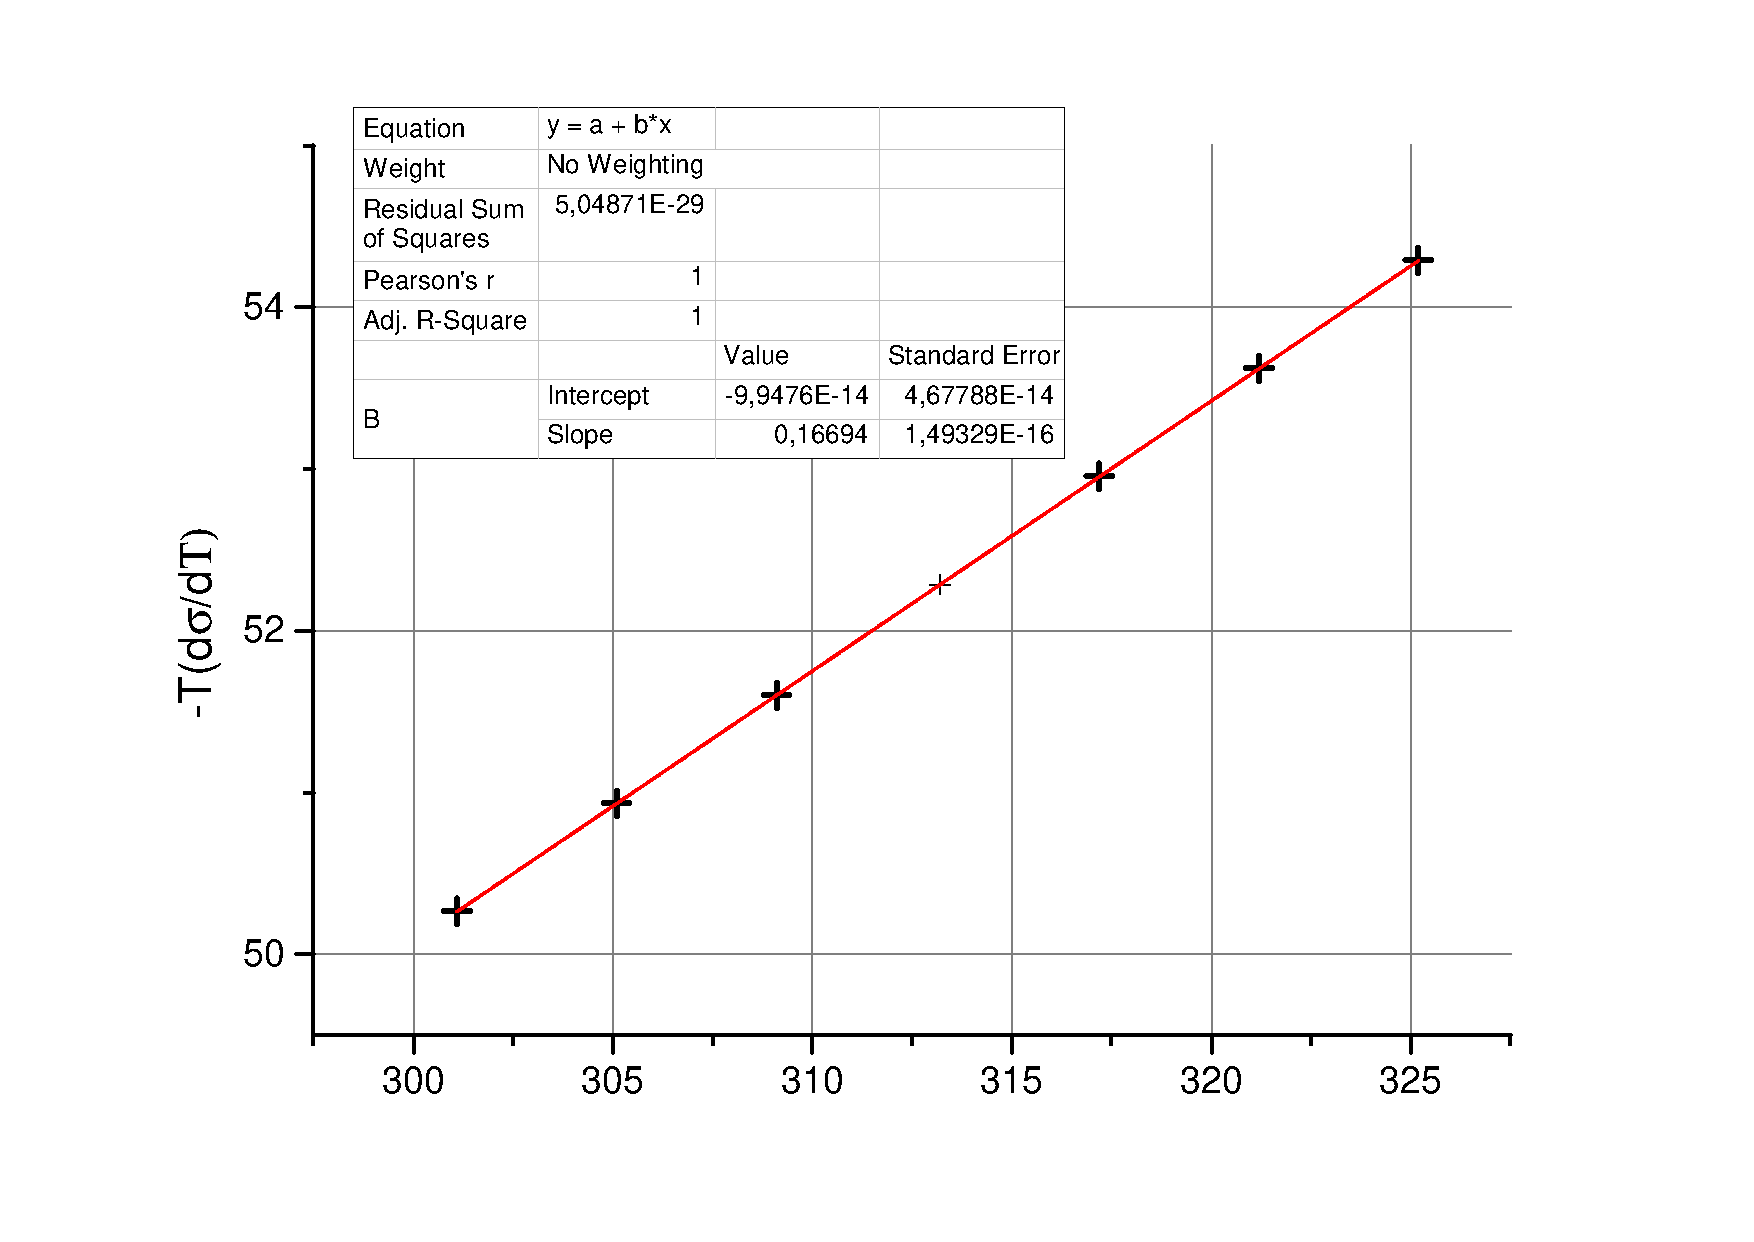
\includegraphics[width = 0.7\linewidth]{TdsigmadT}
	
	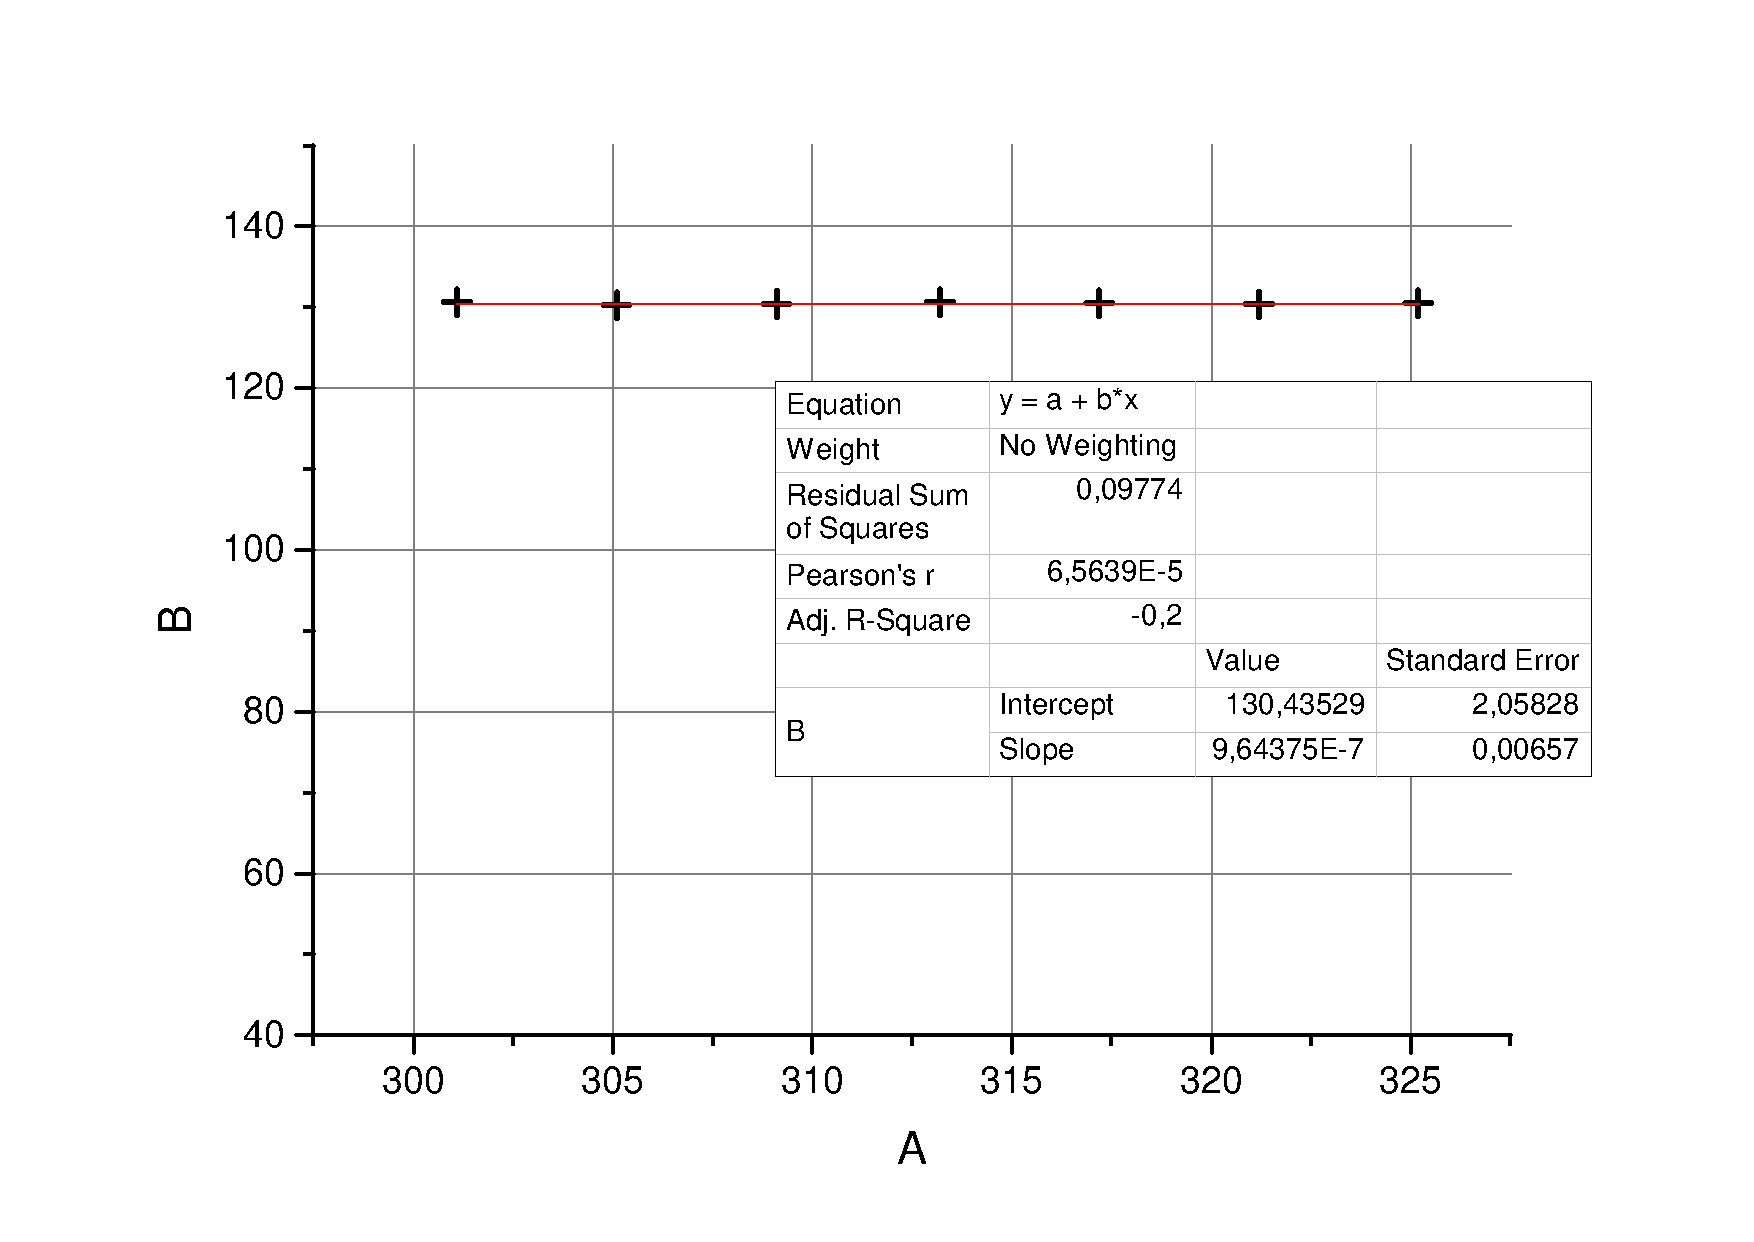
\includegraphics[width = 0.7\linewidth]{Up}
	\section{Вывод}
	Поверхностные эффекты влияют на свойства поверхности, т.к. силы, действующие на поверхностный слой нескомпенсированы. Энергия образования единицы поверхности остается постоянной. 
\end{document}


